% ----------------------------------------------------------------------
%  Pracovní úkoly
% ----------------------------------------------------------------------
\section{Pracovní úkoly}

\begin{enumerate}
\item Určete závislost povrchového napětí \(\sigma\) na objemové koncentraci \(c\) roztoku etylalkoholu ve vodě odtrhávací metodou.

\item Sestrojte graf této závislosti.

\end{enumerate}

% ----------------------------------------------------------------------
%  Teoretická část
% ----------------------------------------------------------------------
\section{Teoretická část}

Povrchovým napětím \(\sigma\) nazýváme kolmou sílu působící na jednotkovou délku na povrch určité látky. Zároveň je tato síla stejná ve všech místech povrchu. Povrchovým napětím se zabýváme zejména u kapalin. Velikost napětí je závislá na teplotě a čistotě kapalin. Látky, které ovlivňují tuto hodnotu, se nazývají povrchově aktivní.

Závislost povrchového napětí na koncentraci budeme měřit tzv. odtrhávací metodou. K měření použijeme torzní váhy, jejichž schéma je znázorněno na obrázku \ref{fig:torzni-vahy}.

\begin{figure}[h]
    \centering
    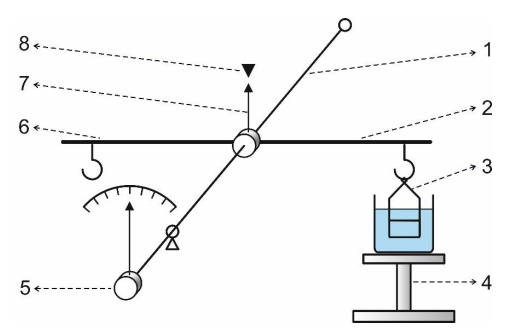
\includegraphics[width=0.5\linewidth]{4 - Závislost povrchového napětí na koncentraci povrchově aktivní látky//Protokol_povrchové napětí//img/Schéma torzních vah.png}
    \caption{Schéma torzních vah}
    \label{fig:torzni-vahy}
\end{figure}

Na pravé straně vah je umístěna nádoba se zkoumanou kapalinou. Do ní je ponořen trámek (3). Na levé straně (6) je umístěno závaží tak, aby byly váhy vyváženy. Nádoba je postupně posouvána dolů (4) a váhy jsou zároveň vyvažovány tak, aby šipka (7) mířila stále na ukazatel (8). V určitý moment je povrchové napětí překonáno a trámek povyskočí směrem vzhůru. V tuto chvíli je zastaveno posouvání a je zaznamenán rozdíl hmotností během zatěžování. Odtud můžeme určit sílu \(P_0\) potřebnou k odtržení trámku.

\begin{equation}
    P_0 = (m_1 - m_2) \cdot g
\end{equation}

kde \(m_1\) a \(m_2\) je počáteční a konečná hmotnost torzních vah a \(g\) gravitační zrychlení. Drátek trámku je je při vytahování z kapaliny držen silou

\begin{equation}
    2F = 2 \sigma \cdot l
\end{equation}

kde \(l\) je délka drátu.

Síla \(P_0\) odpovídá síle \(2F\) a proto dostáváme vztah pro povrchové napětí

\begin{equation}
    \sigma = \frac{(m_1 - m_2)\cdot g}{2l}
\end{equation}

Pro přesnější určení povrchového napětí s korekcí tloušťky drátu použijeme

\begin{equation}
    \sigma = \frac{P_2 - P_1}{2l}-r\Bigg(\sqrt{\frac{(P_2 - P_1)\rho g}{l}}-\frac{P_2 - P_1}{l^2} \Bigg)
\end{equation}

kde \(\rho\) je hustota drátu a \(r\) je poloměr drátu.

% ----------------------------------------------------------------------
%  Výsledky a zpracování měření
% ----------------------------------------------------------------------
\section{Výsledky a zpracování měření}

\subsection{Laboratorní podmínky}

    Měření bylo prováděno za laboratorních podmínek uvedených v tabulce \ref{tab:lab_pod}.

    \begin{table}[h]
        \centering
        \begin{tabular}{|c|c|c|} 
        \hline
            t / °C & p / hPa & vlhkost / \%RH  \\ 
        \hline
            24,0(4)   & 989,2(20)   & 42,0(25)            \\
        \hline
        \end{tabular}
        \caption{Laboratorní podmínky}
        \label{tab:lab_pod}
    \end{table}

\subsection{Podnadpis}

    
% ----------------------------------------------------------------------
%  Diskuse výsledků
% ----------------------------------------------------------------------			
\section{Diskuse výsledků}

% ----------------------------------------------------------------------
%  Závěr
% ----------------------------------------------------------------------
\section{Závěr}
